\chapter{Spikeball}\index{spikeball}\index{roundnet}
\printchapterversion{01_spikeball}

\newthought{Volleyball, Inverted}

\marginnote{%
  \begin{flushright}
  \newthought{Roundnet, commonly Spikeball}\\
  Invented by Jeff Knurek (1989)\\
  Re-launched by Spikeball Inc.\ (2008)\\[4pt]
  {\color{black}\qrcode[height=1.2cm]{https://en.wikipedia.org/wiki/Roundnet}}
  \end{flushright}%
  \bigskip
  \newthought{Why here.}\\
  A game whose entire ruleset fits on a single page, and whose physics demands that you know where everyone is at once.%
}

\marginnote{\newthought{Equipment.} A circular frame roughly 90~cm in diameter with a taut elastic net stretched across it, plus a small inflatable ball about the size of a fist.}

\newthought{Two against two.} Four players stand around a small round trampoline on the ground. A team has up to three touches to return the ball to the net; once it leaves the net the court is 360 degrees and players move freely.

\vspace{1.5em}

\begin{tabular}{p{3.8cm} p{6.5cm}}
    \textbf{Players}   & 2 vs.\ 2. \\[3pt]
    \textbf{Equipment} & Circular net, small inflatable ball. \\[3pt]
    \textbf{Objective} & Hit the ball onto the net so the opponents cannot legally return it. \\[3pt]
    \textbf{Scoring}   & Rally scoring; standard play to 21, win by 2. \\
\end{tabular}

\vspace{1.5em}

\begin{center}
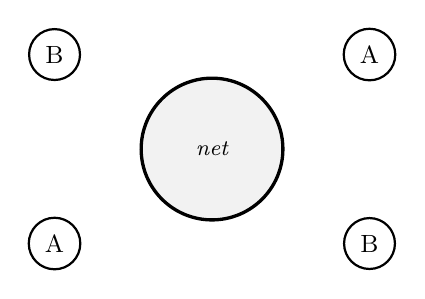
\begin{tikzpicture}[every node/.style={font=\small}]
  \tikzset{
    net/.style={circle, draw, very thick, minimum size=1.8cm, fill=gray!10},
    p/.style={circle, draw, thick, minimum size=0.6cm, fill=white}
  }
  \node[net] (net) at (0,0) {};
  \node[font=\itshape\footnotesize] at (0,0) {net};
  \node[p] at ( 2.0, 1.2) {A};
  \node[p] at (-2.0,-1.2) {A};
  \node[p] at (-2.0, 1.2) {B};
  \node[p] at ( 2.0,-1.2) {B};
\end{tikzpicture}
\end{center}

\vspace{1em}

\marginnote{\newthought{Hinder.} A receiver must be granted a clear path to the ball after the serve. If a server blocks the line of play, the point is replayed without penalty.}

\marginnote{\newthought{Take it from here.} A small ruleset, an asymmetric topology, no walls. The same recipe shows up in much harder problems, just with different balls.}

\newthought{Faults end the rally:} more than three touches, the ball striking the rim instead of the net, a return that fails to clear the rim, or a double touch by a single player. Game ends at the target score with a margin of two.
